\index{A simple graph}
\begin{center}
% \usetikzlibrary{shadows}
% \usetikzlibrary{arrows.meta, arrows}

	\tikzset{myNode/.style={draw, circle, white, radius=2pt, top color=red!40, bottom color=red!100, circular drop shadow={black!30}}, myEdge/.style={-{Stealth[open, round]}, very thick, green}} % thin, thick, very thick, fill=color_name removed. font=\itshape or \ttfamily.
	\tikz
	{
		% Vertices
		\node(Y) [myNode] at (2, 1) {\textbf{Y}};
		\node(X) [myNode] at (-2, 1) {\textbf{X}};
		\node(T) [myNode] at (-2, -1) {\textbf{T}};
		\node(S) [myNode] at (2, -1) {\textbf{S}};
		
		% Edges
		\draw[myEdge] (Y) to node[auto, swap, black, font=\ttfamily] {\textbf{3}} (X);
		\draw[myEdge] (Y) to node(2) [auto, black, font=\ttfamily] {\textbf{2}} (S);
		\draw[myEdge] (T) to node[auto, black, font=\ttfamily] {\textbf{4}} (S);
		\draw[myEdge] (T) to node[auto, black, font=\ttfamily] {\textbf{6}} (X);
		\draw[myEdge] (T) to node[auto, black, font=\ttfamily] {\textbf{1}} (Y);
		\draw[myEdge] (X) to[out=40, in=90+50] node[auto, black, font=\ttfamily] {\textbf{7}} (Y);
		\draw[myEdge] (S) to[out=-140, in=-40] node[auto, swap, black, font=\ttfamily] {\textbf{5}} (T);
		
		\node[draw, black, right=1cm, text width=6cm, font=\itshape, fill=green!10] at (2) {\textbf{Find out the shortest path of this graph using Warshall's algorithm.}};
	}

\end{center}

%\begin{figure}[hbtp]
%\centering
%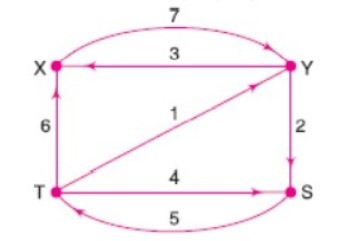
\includegraphics[scale=0.5]{Pictures/Screenshot_2.jpg}
%\caption{A directed graph}
%\end{figure}

\index{Weight matrix illustration}
\subsection{Weight matrix}
$$
\textrm{Weight matrix of G, W }=
\begin{Vmatrix}
	  & X & Y & S & T\\
	X & 0 & 7 & 0 & 0 \\
	Y & 3 & 0 & 2 & 0 \\
	S & 0 & 0 & 0 & 5 \\
	T & 6 & 1 & 4 & 0 \\
\end{Vmatrix}
$$
	
\subsection{Finding shortest path using Warshall's algorithm}
\index{Warshall's algorithm illustration}
$$
Q_0=
\begin{bmatrix}
	0 & 7 & \infty & \infty \\
	3 & 0 & 2 & \infty \\
	\infty & \infty & 0 & 5 \\
	6 & 1 & 4 & 0 \\
\end{bmatrix}
$$
\vspace{0.5cm}
$$
Q_X=
\begin{bmatrix}
0 & 7 & \infty & \infty \\
3 & 0 & 2 & \infty \\
\infty & \infty & 0 & 5 \\
6 & 1 & 4 & 0 \\
\end{bmatrix}
\hspace{2cm}
Q_Y=
\begin{bmatrix}
0 & 7 & 9 & \infty \\
3 & 0 & 2 & \infty \\
\infty & \infty & 0 & 5 \\
4 & 1 & 3 & 0 \\
\end{bmatrix}
$$
\vspace{0.5cm}
$$
Q_S=
\begin{bmatrix}
0 & 7 & 9 & \infty \\
3 & 0 & 2 & 7 \\
\infty & 0 & 0 & 5 \\
4 & 1 & 3 & 0 \\
\end{bmatrix}
\hspace{2cm}
Q_T=
\begin{bmatrix}
0 & 7 & 9 & \infty \\
3 & 0 & 2 & 7 \\
11 & 6 & 0 & 5 \\
4 & 1 & 3 & 0 \\
\end{bmatrix}
$$

Ultimately the shortest path: 
$
\textrm{Q}=
\begin{Vmatrix}
0 & 7 & 9 & \infty \\
3 & 0 & 2 & 7 \\
11 & 6 & 0 & 5 \\
4 & 1 & 3 & 0 \\
\end{Vmatrix}
$